\documentclass{standalone}
\usepackage{tikz}
\usetikzlibrary{shapes.geometric, arrows}

\tikzstyle{startstop} = [rectangle, rounded corners, 
minimum width=3cm, 
minimum height=1cm,
text centered, 
draw=black, 
fill=red!30]

\tikzstyle{io} = [trapezium, 
trapezium stretches=true, % A later addition
trapezium left angle=70, 
trapezium right angle=110, 
minimum width=3cm, 
minimum height=1cm, text centered, 
draw=black, fill=blue!30]

\tikzstyle{process} = [rectangle, 
minimum width=3cm, 
minimum height=1cm, 
text centered, 
text width=3cm, 
draw=black, 
fill=orange!30]

\tikzstyle{decision} = [diamond, 
minimum width=3cm, 
minimum height=1cm, 
text centered, 
draw=black, 
fill=green!30]
\tikzstyle{arrow} = [thick,->,>=stealth]
\begin{document}

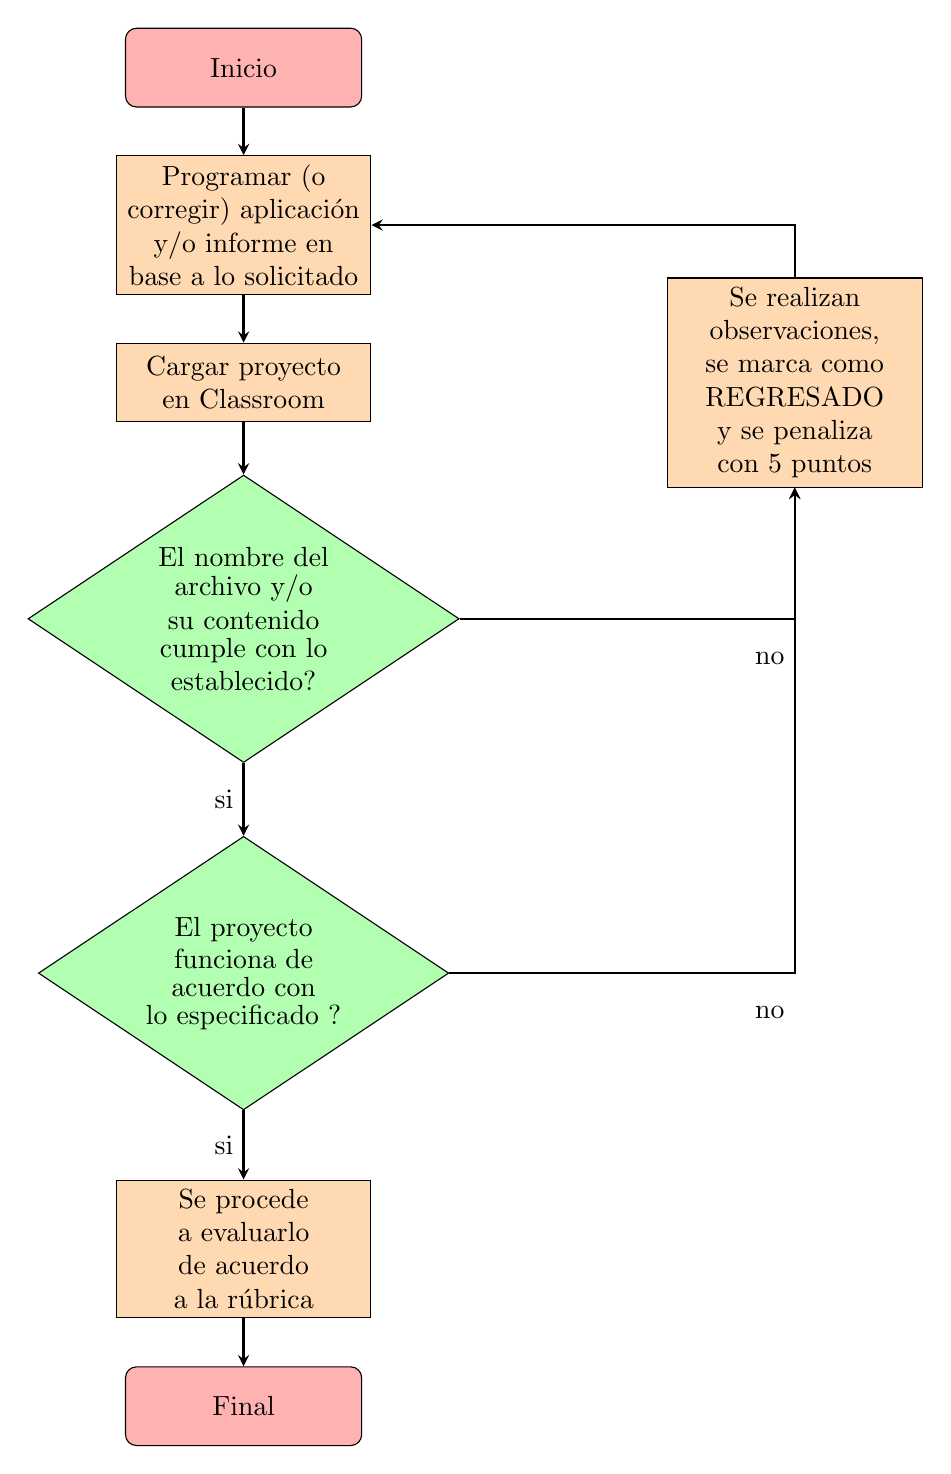
\begin{tikzpicture}[node distance=2.0cm]

\node (start) [startstop] {Inicio};
%\node (in1) [io, below of=start] {Input};
\node (prot1) [process, below of=start] {Programar (o corregir) aplicaci\'on y/o informe en base a lo solicitado};

\node (pro1) [process, below of=prot1] {Cargar proyecto en Classroom};

%\node (dec1) [decision, below of=pro1, yshift=-0.0cm, aspect=3, label=center:Funciona correctamente?] {};
\node (dec1) [decision, below of=pro1, yshift=-1.0cm, aspect=1.5] { \shortstack{El nombre del \\ archivo y/o\\ su contenido  \\ cumple con lo \\establecido?} };

%\node (dec2) [decision, left of=dec1, xshift=-5.0cm, aspect=2] {El nombre del archivo y/o \\ su contenido cumple con lo establecido?};
\node (dec2) [decision, below of=dec1, yshift=-2.5cm, aspect=1.5] { \shortstack{El proyecto\\ funciona  de \\acuerdo con \\lo especificado ?}  };

\node (pro2a) [process, below of=dec2, yshift=-1.5cm] {Se procede a evaluarlo de acuerdo a la r\'ubrica};

\node (pro2b) [process, right of=pro1, xshift=5cm] {Se realizan observaciones, se marca como REGRESADO y se penaliza con 5 puntos};
%\node (out1) [io, below of=pro2a] {Output};
\node (stop) [startstop, below of=pro2a] {Final};

\draw [arrow] (start) -- (prot1);
\draw [arrow] (prot1) -- (pro1);
\draw [arrow] (pro1) -- (dec1);
\draw [arrow] (dec1) -- node[anchor=east] {si} (dec2);
\draw [arrow] (dec1) -| node[anchor=east,yshift=-0.5cm] {no} (pro2b);

\draw [arrow] (dec2) -- node[anchor=east] {si} (pro2a);
\draw [arrow] (dec2) -| node[anchor=east,yshift=-0.5cm] {no} (pro2b);


%\draw [arrow] (pro2b) |- (prot1);
%\draw [arrow] (pro2b) |- node[anchor=north] {} (pro1);
\draw [arrow] (pro2b) |- (prot1);
\draw [arrow] (pro2a) -- (stop);
%\draw [arrow] (out1) -- (stop);

\end{tikzpicture}
\end{document}
